% Editable vector reconstruction of the supplied figure.
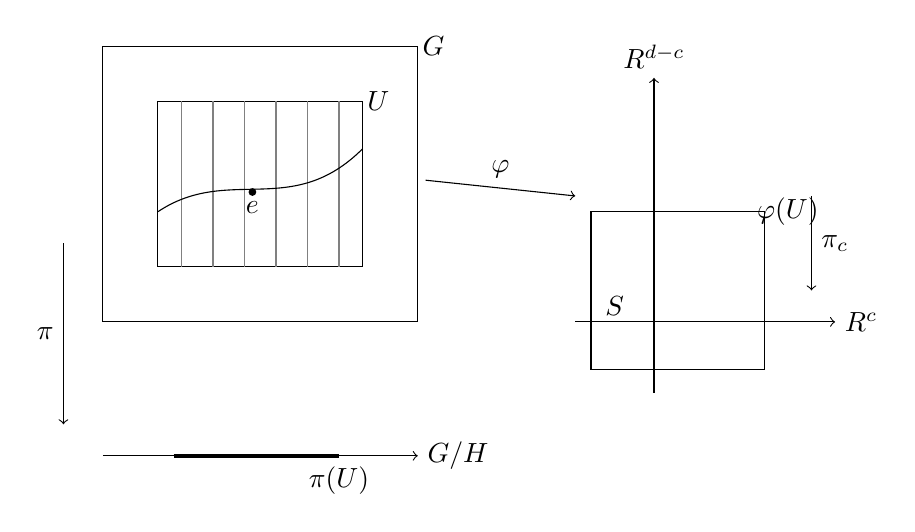
\begin{tikzpicture}
\draw(0,0)rectangle(4,3.5);\node at(4.2,3.5){$G$};\draw(.7,.7)rectangle(3.3,2.8);\node at(3.5,2.8){$U$};\foreach \a in {1,1.4,...,3}{\draw[gray](\a,.7)--(\a,2.8);}\draw(.7,1.4)..controls(1.6,2)and(2.4,1.3)..(3.3,2.2);\fill(1.9,1.65)circle(1.4pt)node[below]{$e$};\draw[->](4.1,1.8)--node[above]{$\varphi$}(6,1.6);
\draw[->](6,0)--(9.3,0)node[right]{$\mathbb R^c$};\draw[->](7,-.9)--(7,3.1)node[above]{$\mathbb R^{d-c}$};\draw(6.2,-.6)rectangle(8.4,1.4);\node at(8.7,1.4){$\varphi(U)$};\node at(6.5,.2){$S$};\draw[->](9,1.6)--node[right]{$\pi_c$}(9,.4);
\draw[->](-.5,1)--node[left]{$\pi$}(-.5,-1.3);\draw[->](0,-1.7)--(4,-1.7)node[right]{$G/H$};\draw[line width=1.3pt](.9,-1.7)--(3,-1.7)node[below]{$\pi(U)$};
\end{tikzpicture}
